\documentclass[a4paper,12pt]{article}
\usepackage[utf8]{inputenc}
\usepackage{amsmath, amssymb}
\usepackage{graphicx}
\usepackage{float}
\usepackage{tikz}
\usepackage{listings}
\usepackage{xcolor}
\usepackage{caption}
\usepackage{geometry}
\usepackage{fancyhdr} % Added for headers
\geometry{margin=1in}

\title{Big Assignment: Object-Oriented Programming\\\large Project Design Document\\(part 2)}
\author{Yusupov Boburjon\\Neptun Code: YTAJDI}
\date{May 1, 2025}
\captionsetup[figure]{labelformat=empty}

\pagestyle{fancy}
\fancyhf{}
\fancyhead[R]{Big Assignment: Object-Oriented Programming (part 2)}
\fancyfoot[C]{\thepage}

\begin{document}

\maketitle

\newpage

\section{\textbf{Additional functionality}}

To introduce more unpredictability of the wild, the simulation includes animal behavior and ranger response patterns to handle high-risk encounters and medical urgency.
Every animal now has a temperament profile — Passive, Defensive, Curious, or Aggressive — which will influence the animal’s reaction when approached. Aggressive animals attack or flee and stress surrounding animals. Defensive animals only defend themselves when cornered, and Curious animals will approach rangers uninvited. Temperament influences how rangers must prepare and interact.
The system also tracks ranger stress, which builds up while conducting dangerous rescues or poacher encounters. If stress becomes too great, the ranger will slow down or make more dangerous choices. Trucks now also have tranquilizer kits or mobile medic units as optional equipment during an emergency, depending on truck type.

\section{\textbf{Animal state diagram}}

The state diagram represents the behavior of the animal throughout the interaction with a ranger. The animals begin in a Calm state. As the ranger approaches, depending on their disposition (temperament profile), they might enter an Alerted, Defensive, Curious, or Aggressive state. While threatened or injured, they might enter Fleeing or Attacking states. Successfully administered treatment brings the animal to a Stabilized state, but severe injury or increasing stress can bring it to a Critical state that requires immediate attention.

\section{\textbf{Scenarios to model with sequence diagrams}}
\subsection{Scenario 1: Hostile Animal Encounter}

A ranger attempts to administer treatment to an injured animal with an Aggressive profile. The animal bites when the ranger gets close, so the ranger retreats and calls for help. Stress is increased, and the habitat is shut down as unsafe for a short period of time.

\subsection{Scenario 2: Emergency Treatment in the Field}
An attack by poachers leaves an animal critically injured. A ranger comes in a vehicle equipped with a med unit and speeds to the animal’s rescue right away. The animal is stabilized right there and is driven directly to the rehabilitation zone by the vehicle.

\newpage

\section{\textbf{Class diagrams}}
\textbf{Updated class diagrams of the simulation.}
The class diagrams show the updated structure of the simulation, including the new fields of classes and relationships introduced in the second part of the assignment. The diagrams illustrate how the classes interact with each other and how they are organized within the system.
\begin{figure}[H]
    \centering
    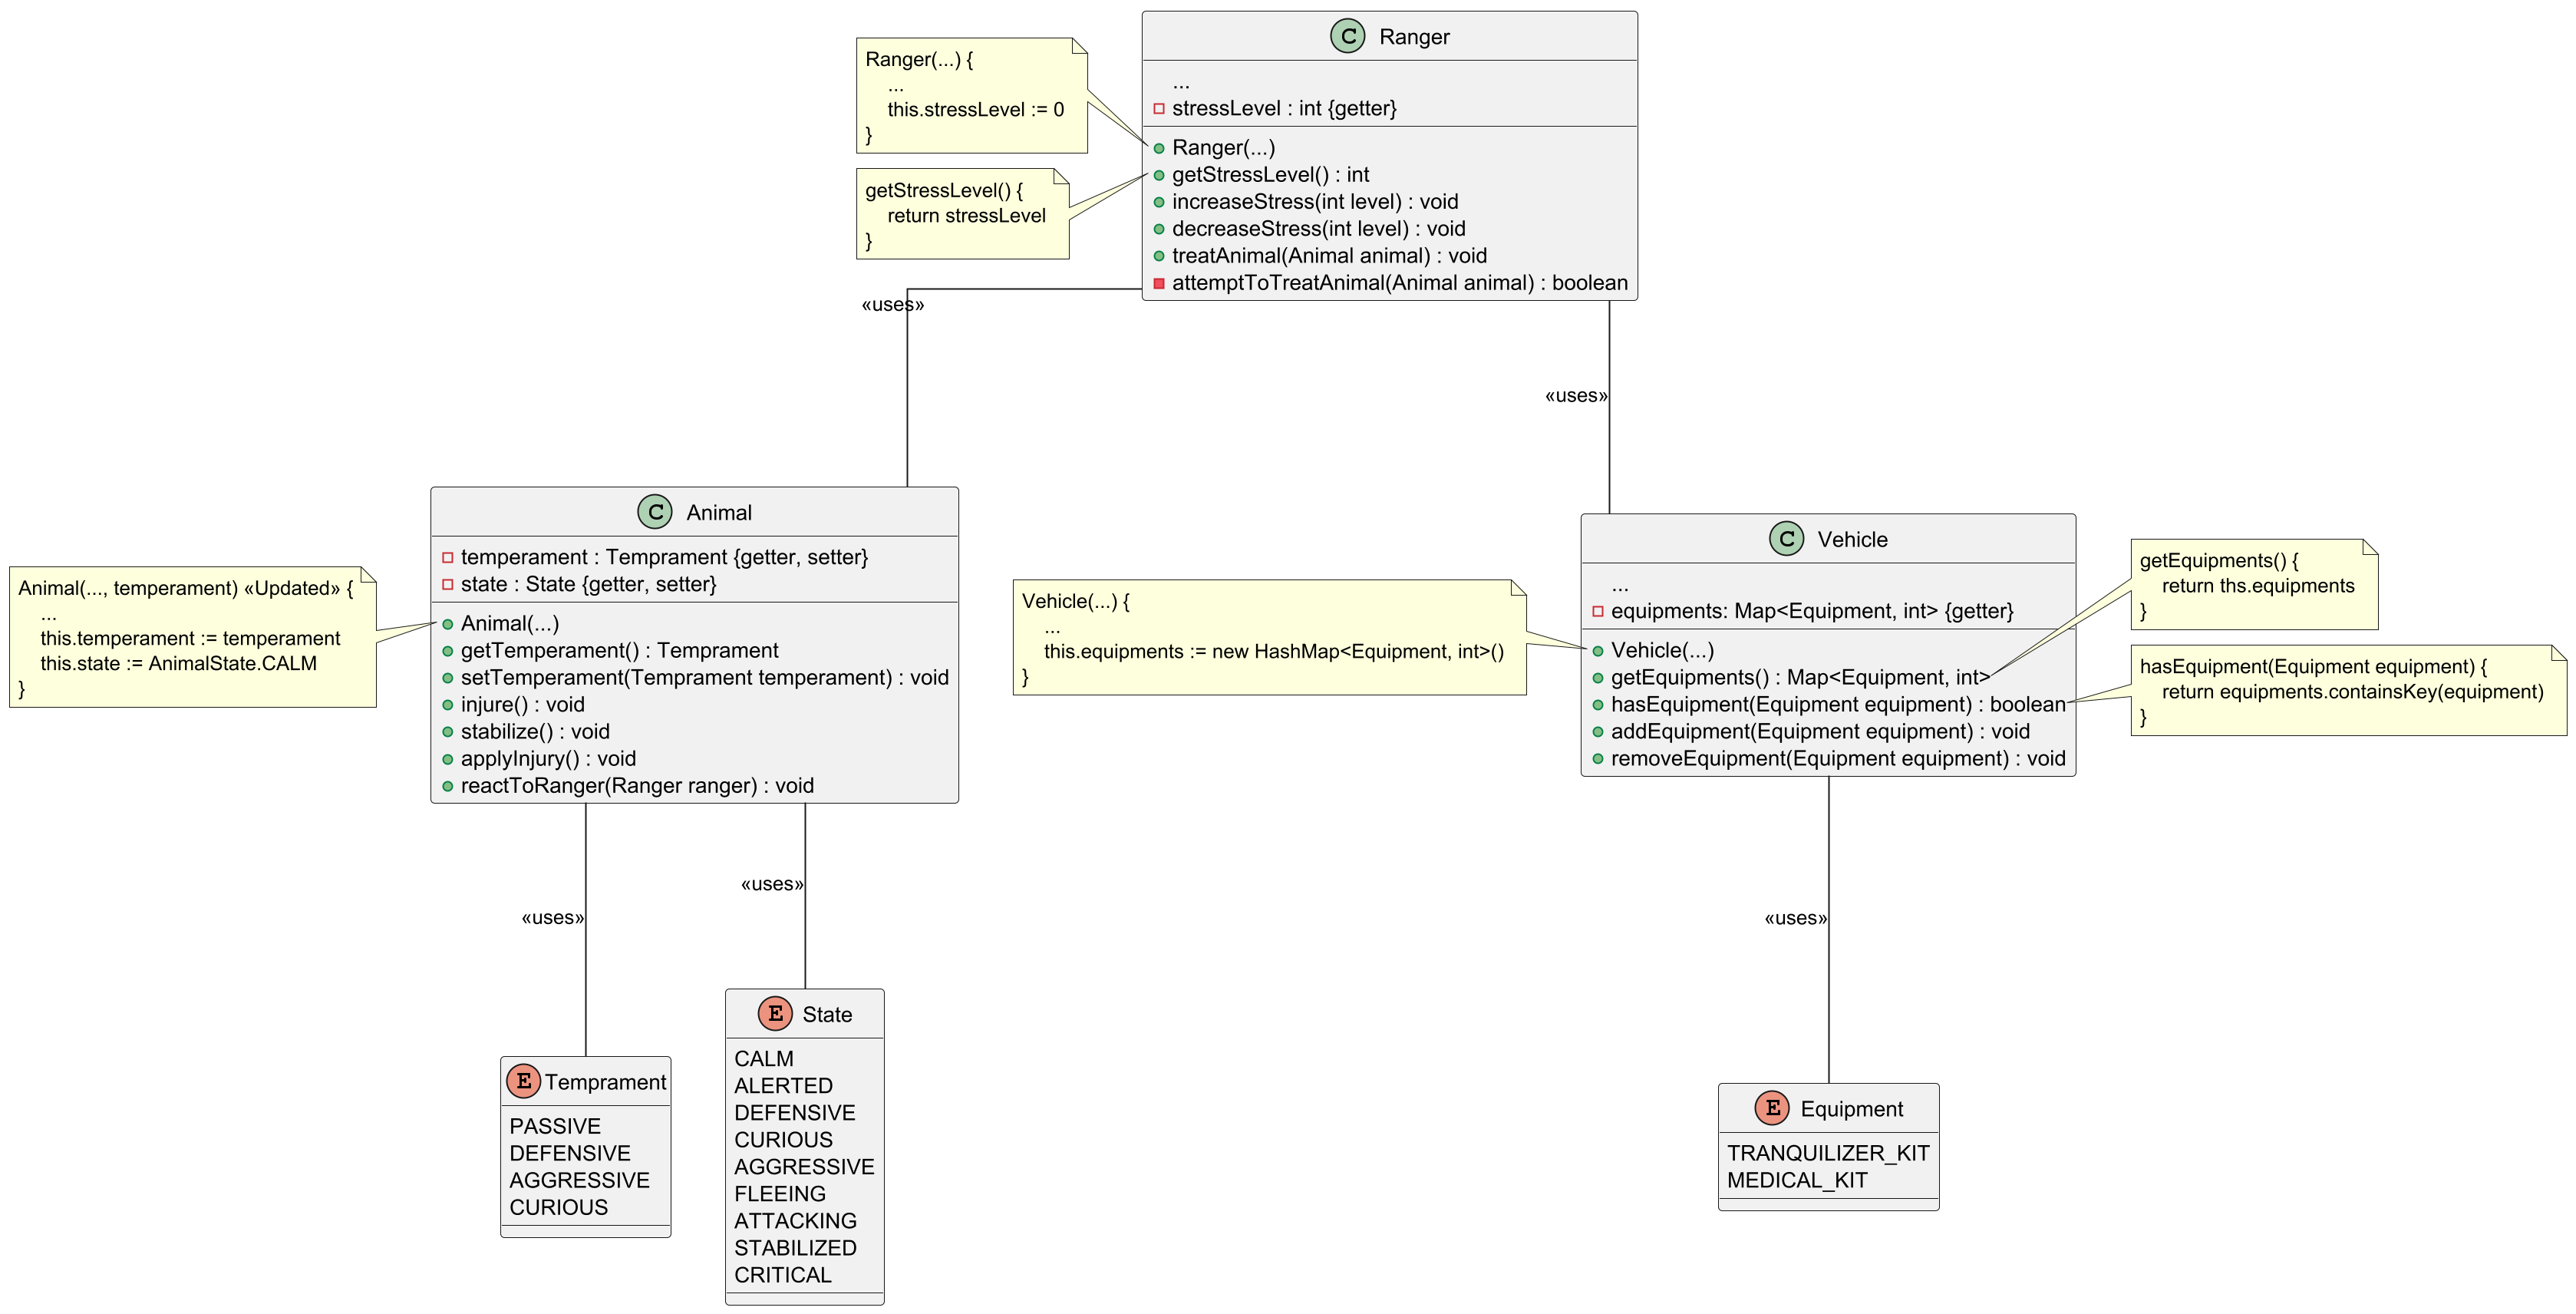
\includegraphics[width=0.8\textwidth]{class-diagram1.png}
    \caption{Class diagram 1}
    \label{fig:class-diagram1}
\end{figure}

\begin{figure}[H]
    \centering
    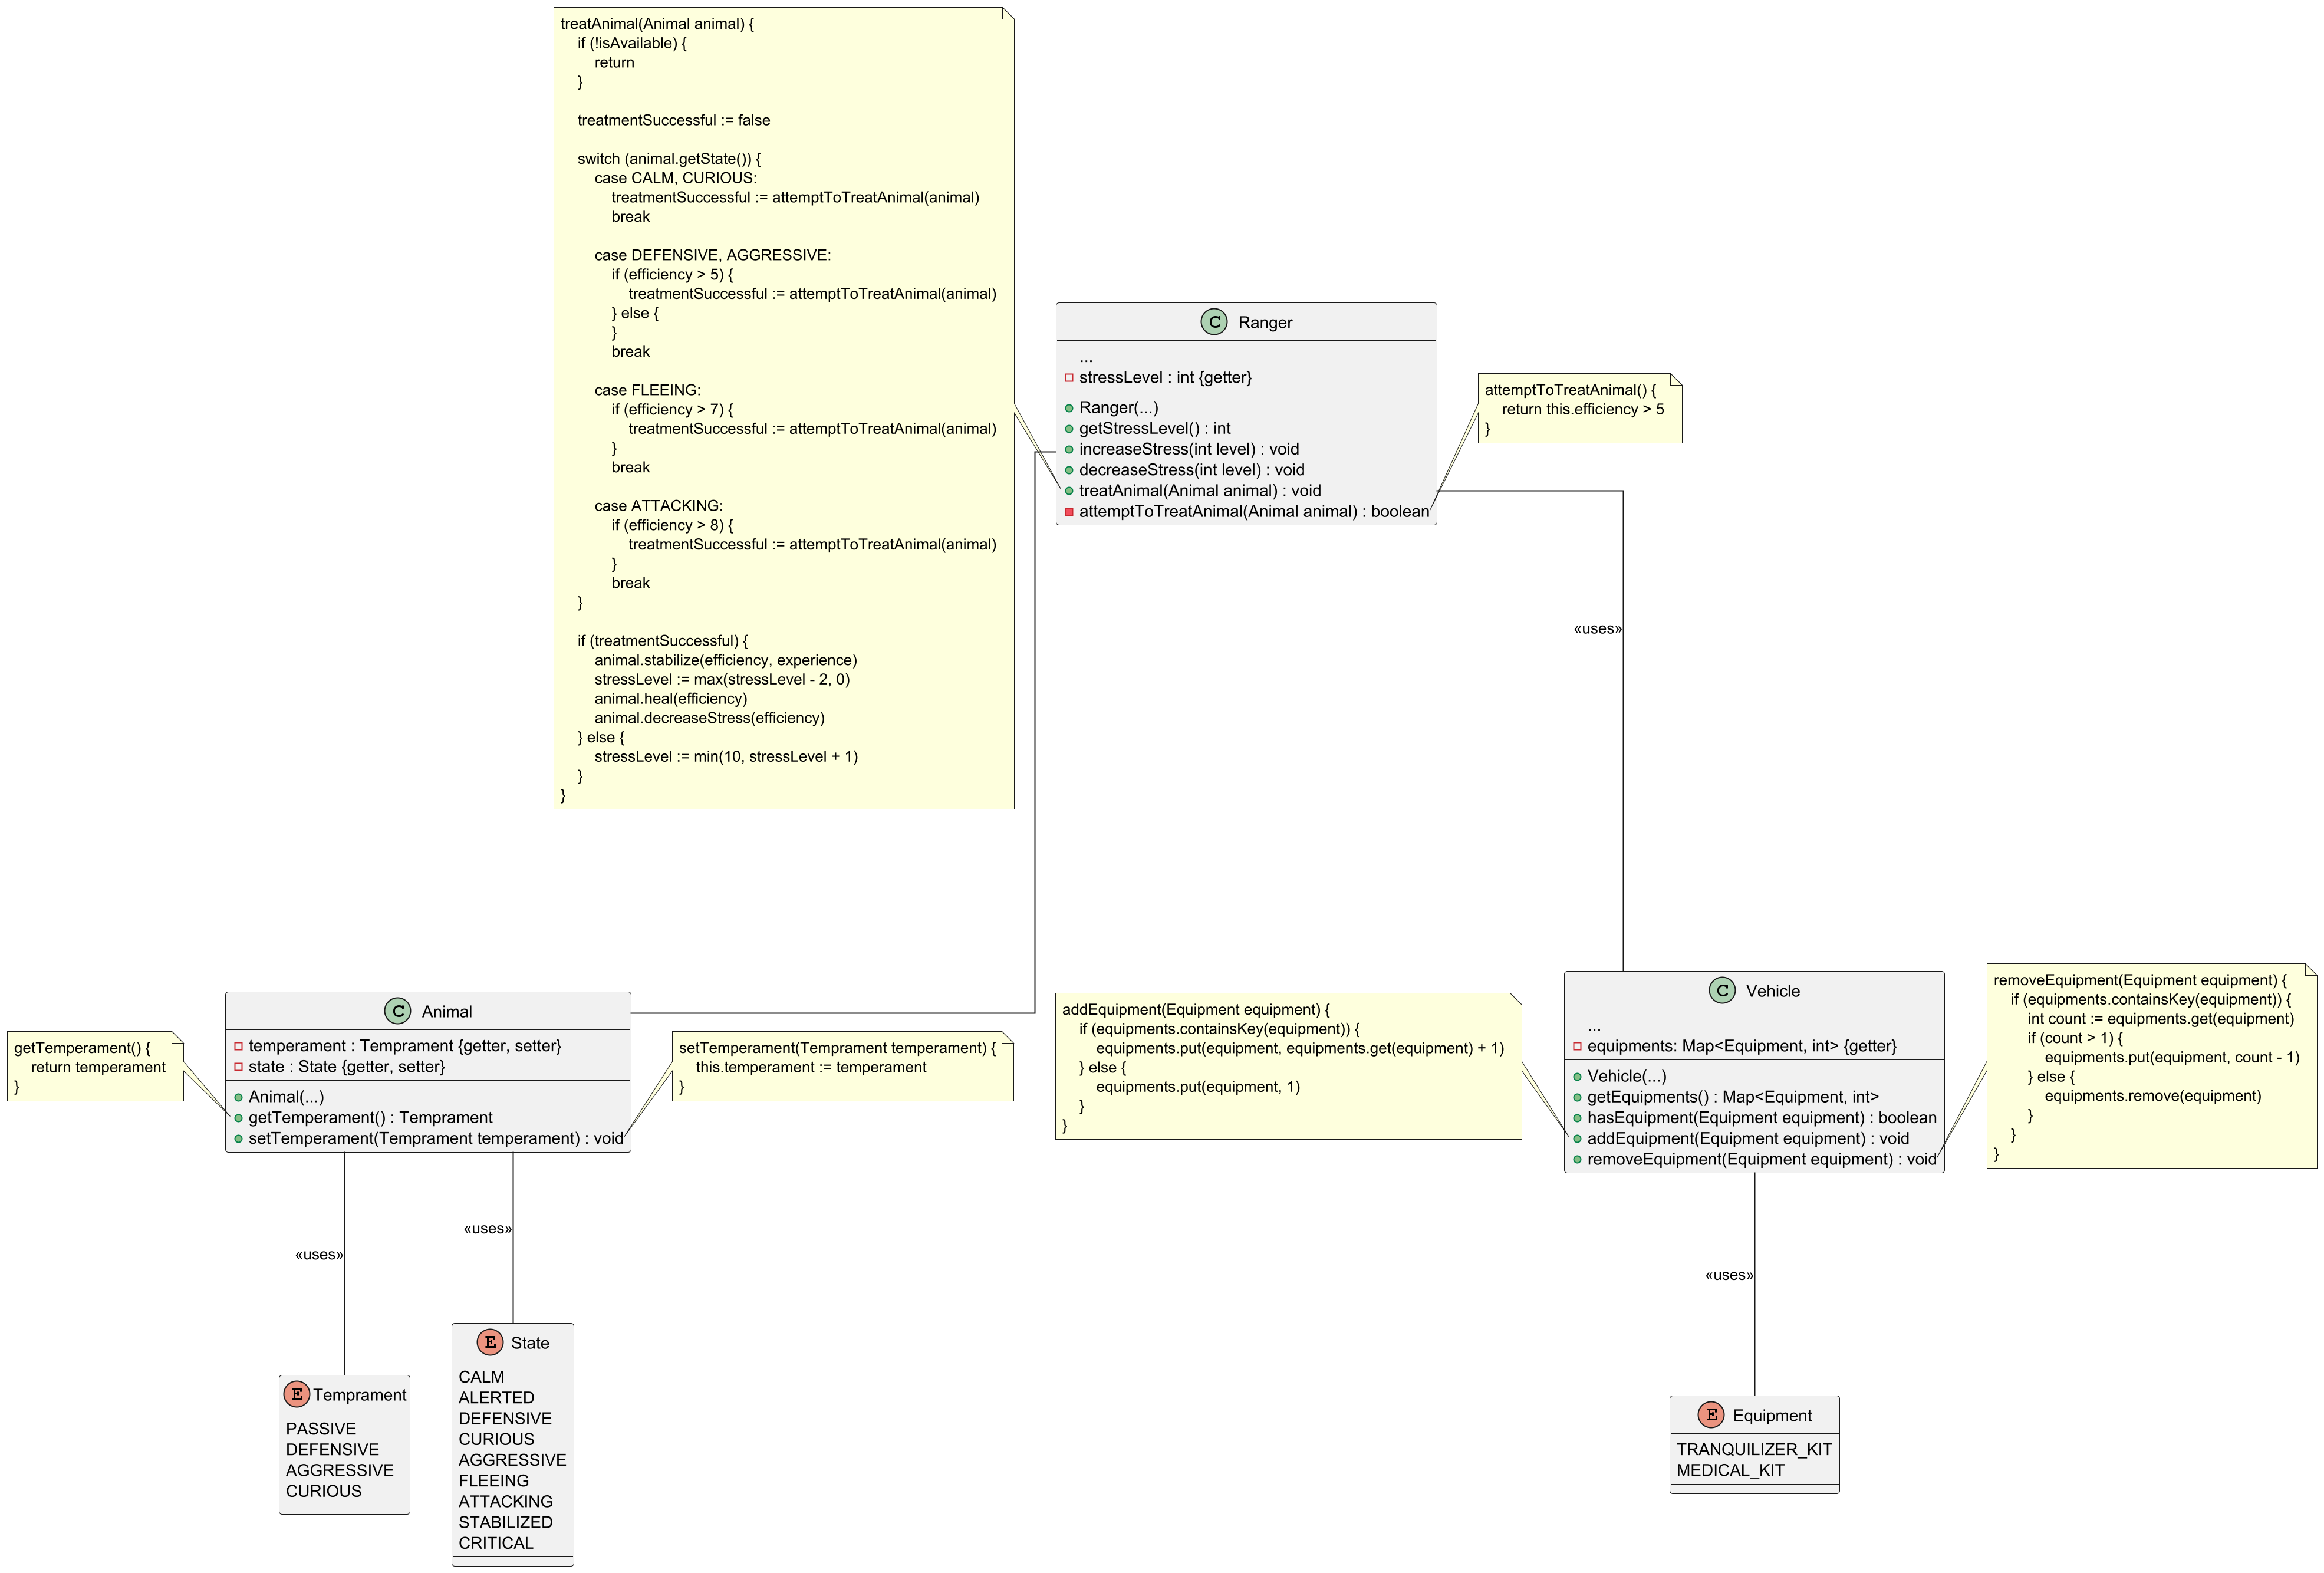
\includegraphics[width=0.9\textwidth]{class-diagram2.png}
    \caption{Class diagram 2}
    \label{fig:class-diagram2}
\end{figure}

\newpage
\section{\textbf{Sequence diagrams}}
\subsection{Scenario 1: Hostile Animal Encounter}
\begin{figure}[H]
    \centering
    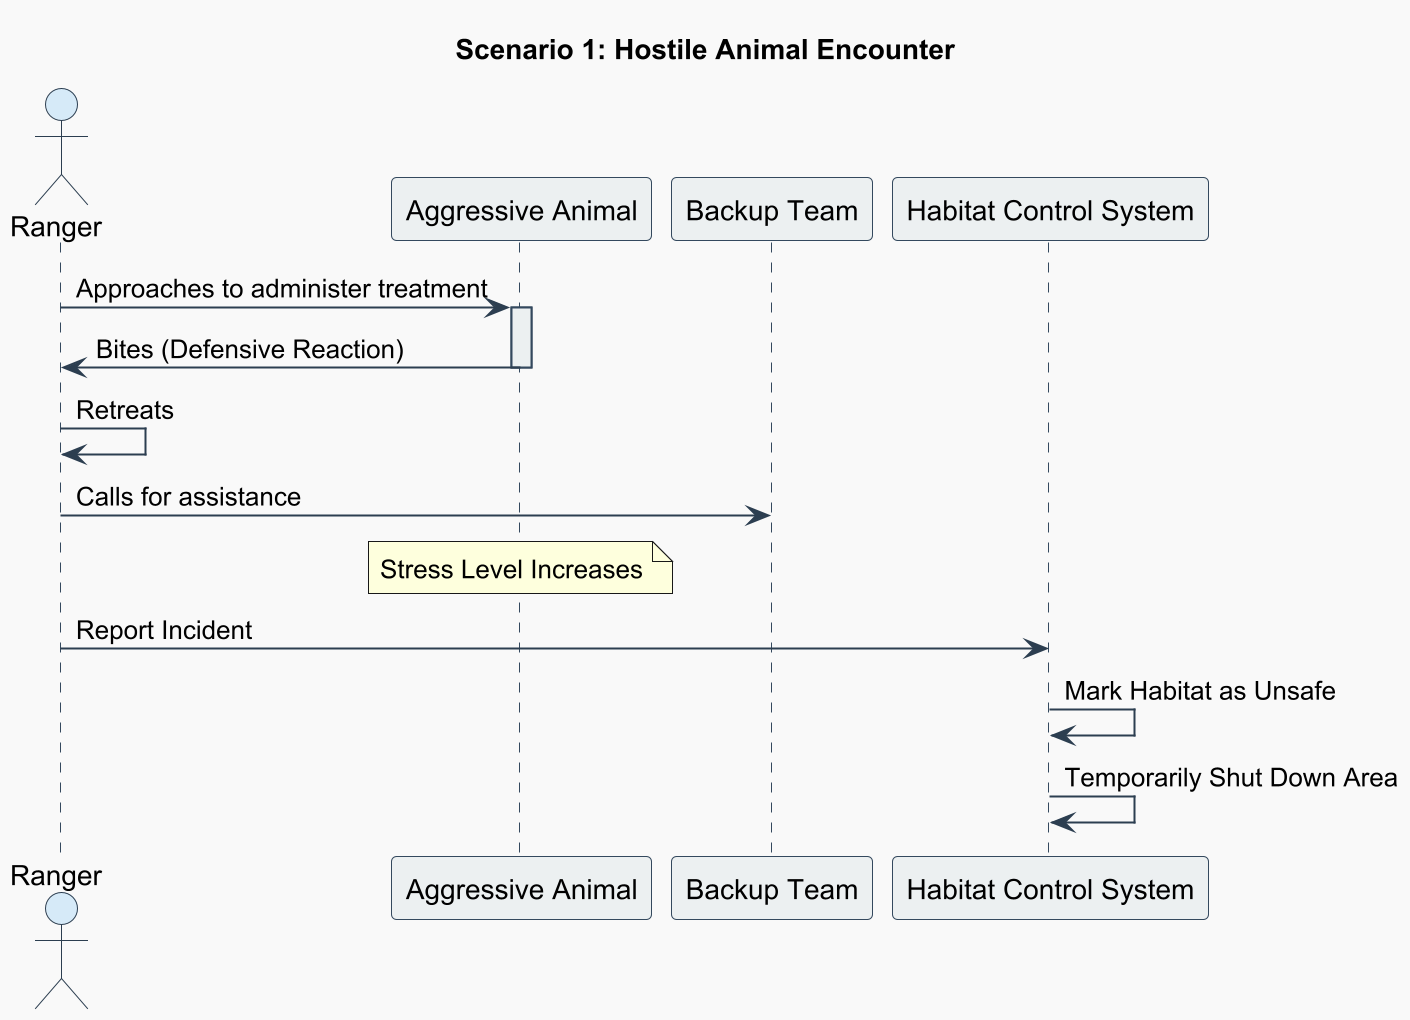
\includegraphics[width=0.8\textwidth]{sequence1.png}
    \caption{Sequence diagram 1}
    \label{fig:sequence-diagram1}
\end{figure}

\subsection{Scenario 2: Emergency Treatment in the Field}
\begin{figure}[H]
    \centering
    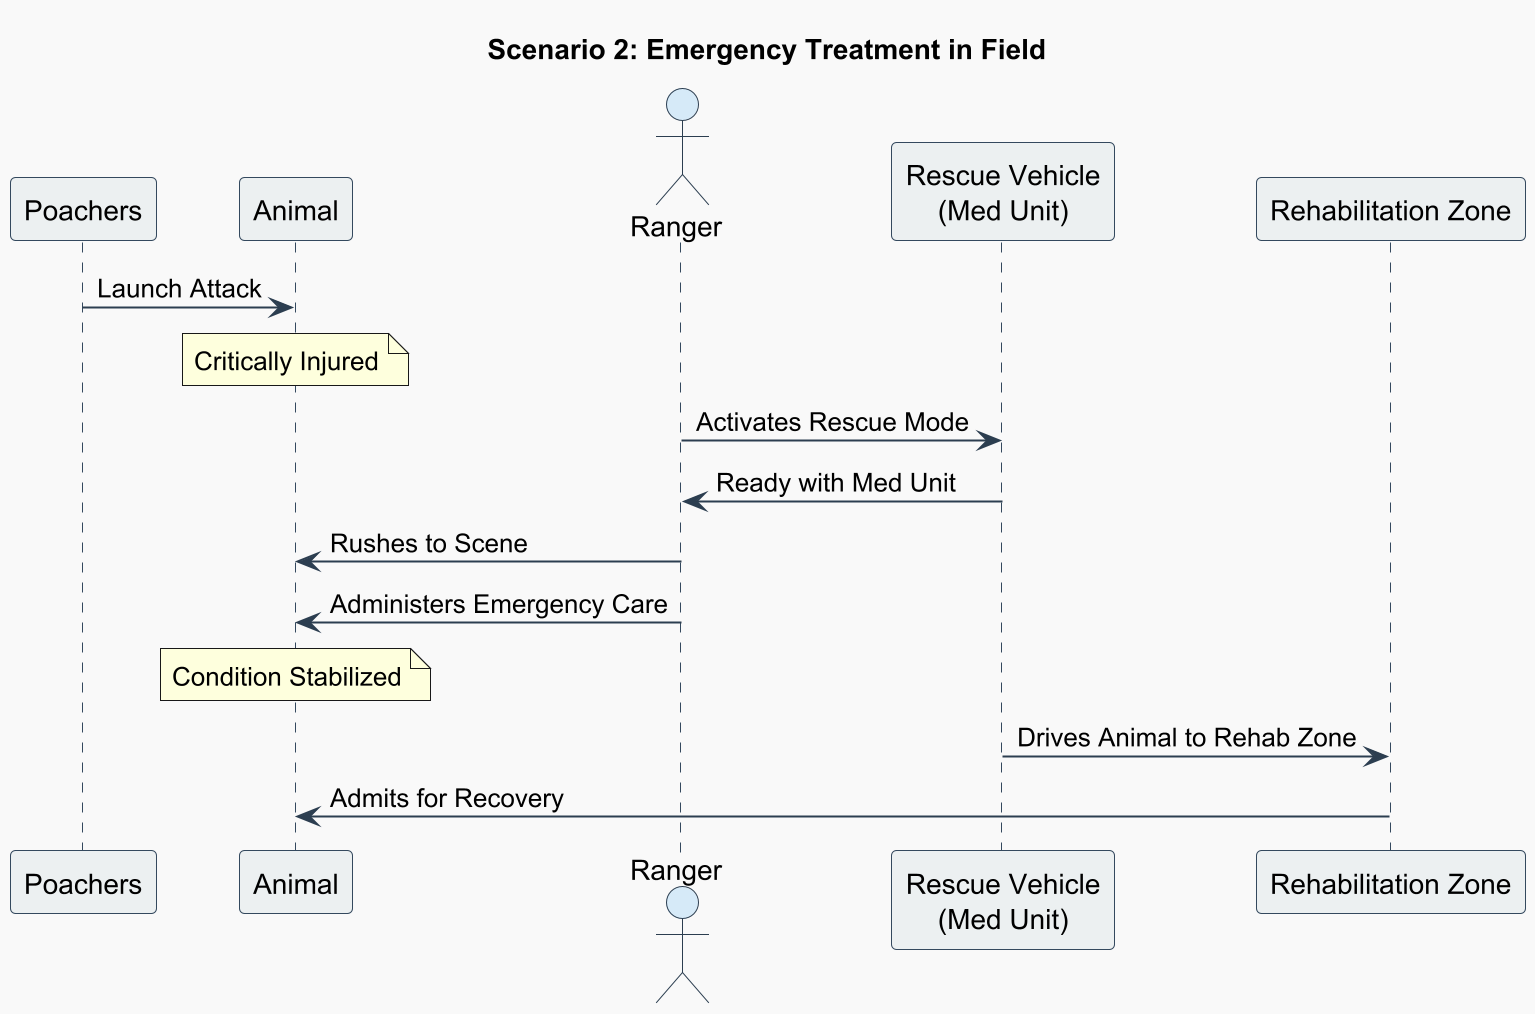
\includegraphics[width=0.8\textwidth]{sequence2.png}
    \caption{Sequence diagram 2}
    \label{fig:sequence-diagram2}
\end{figure}

\newpage
\section{\textbf{State diagrams}}
\subsection{Animal State Diagram}
\begin{figure}[H]
    \centering
    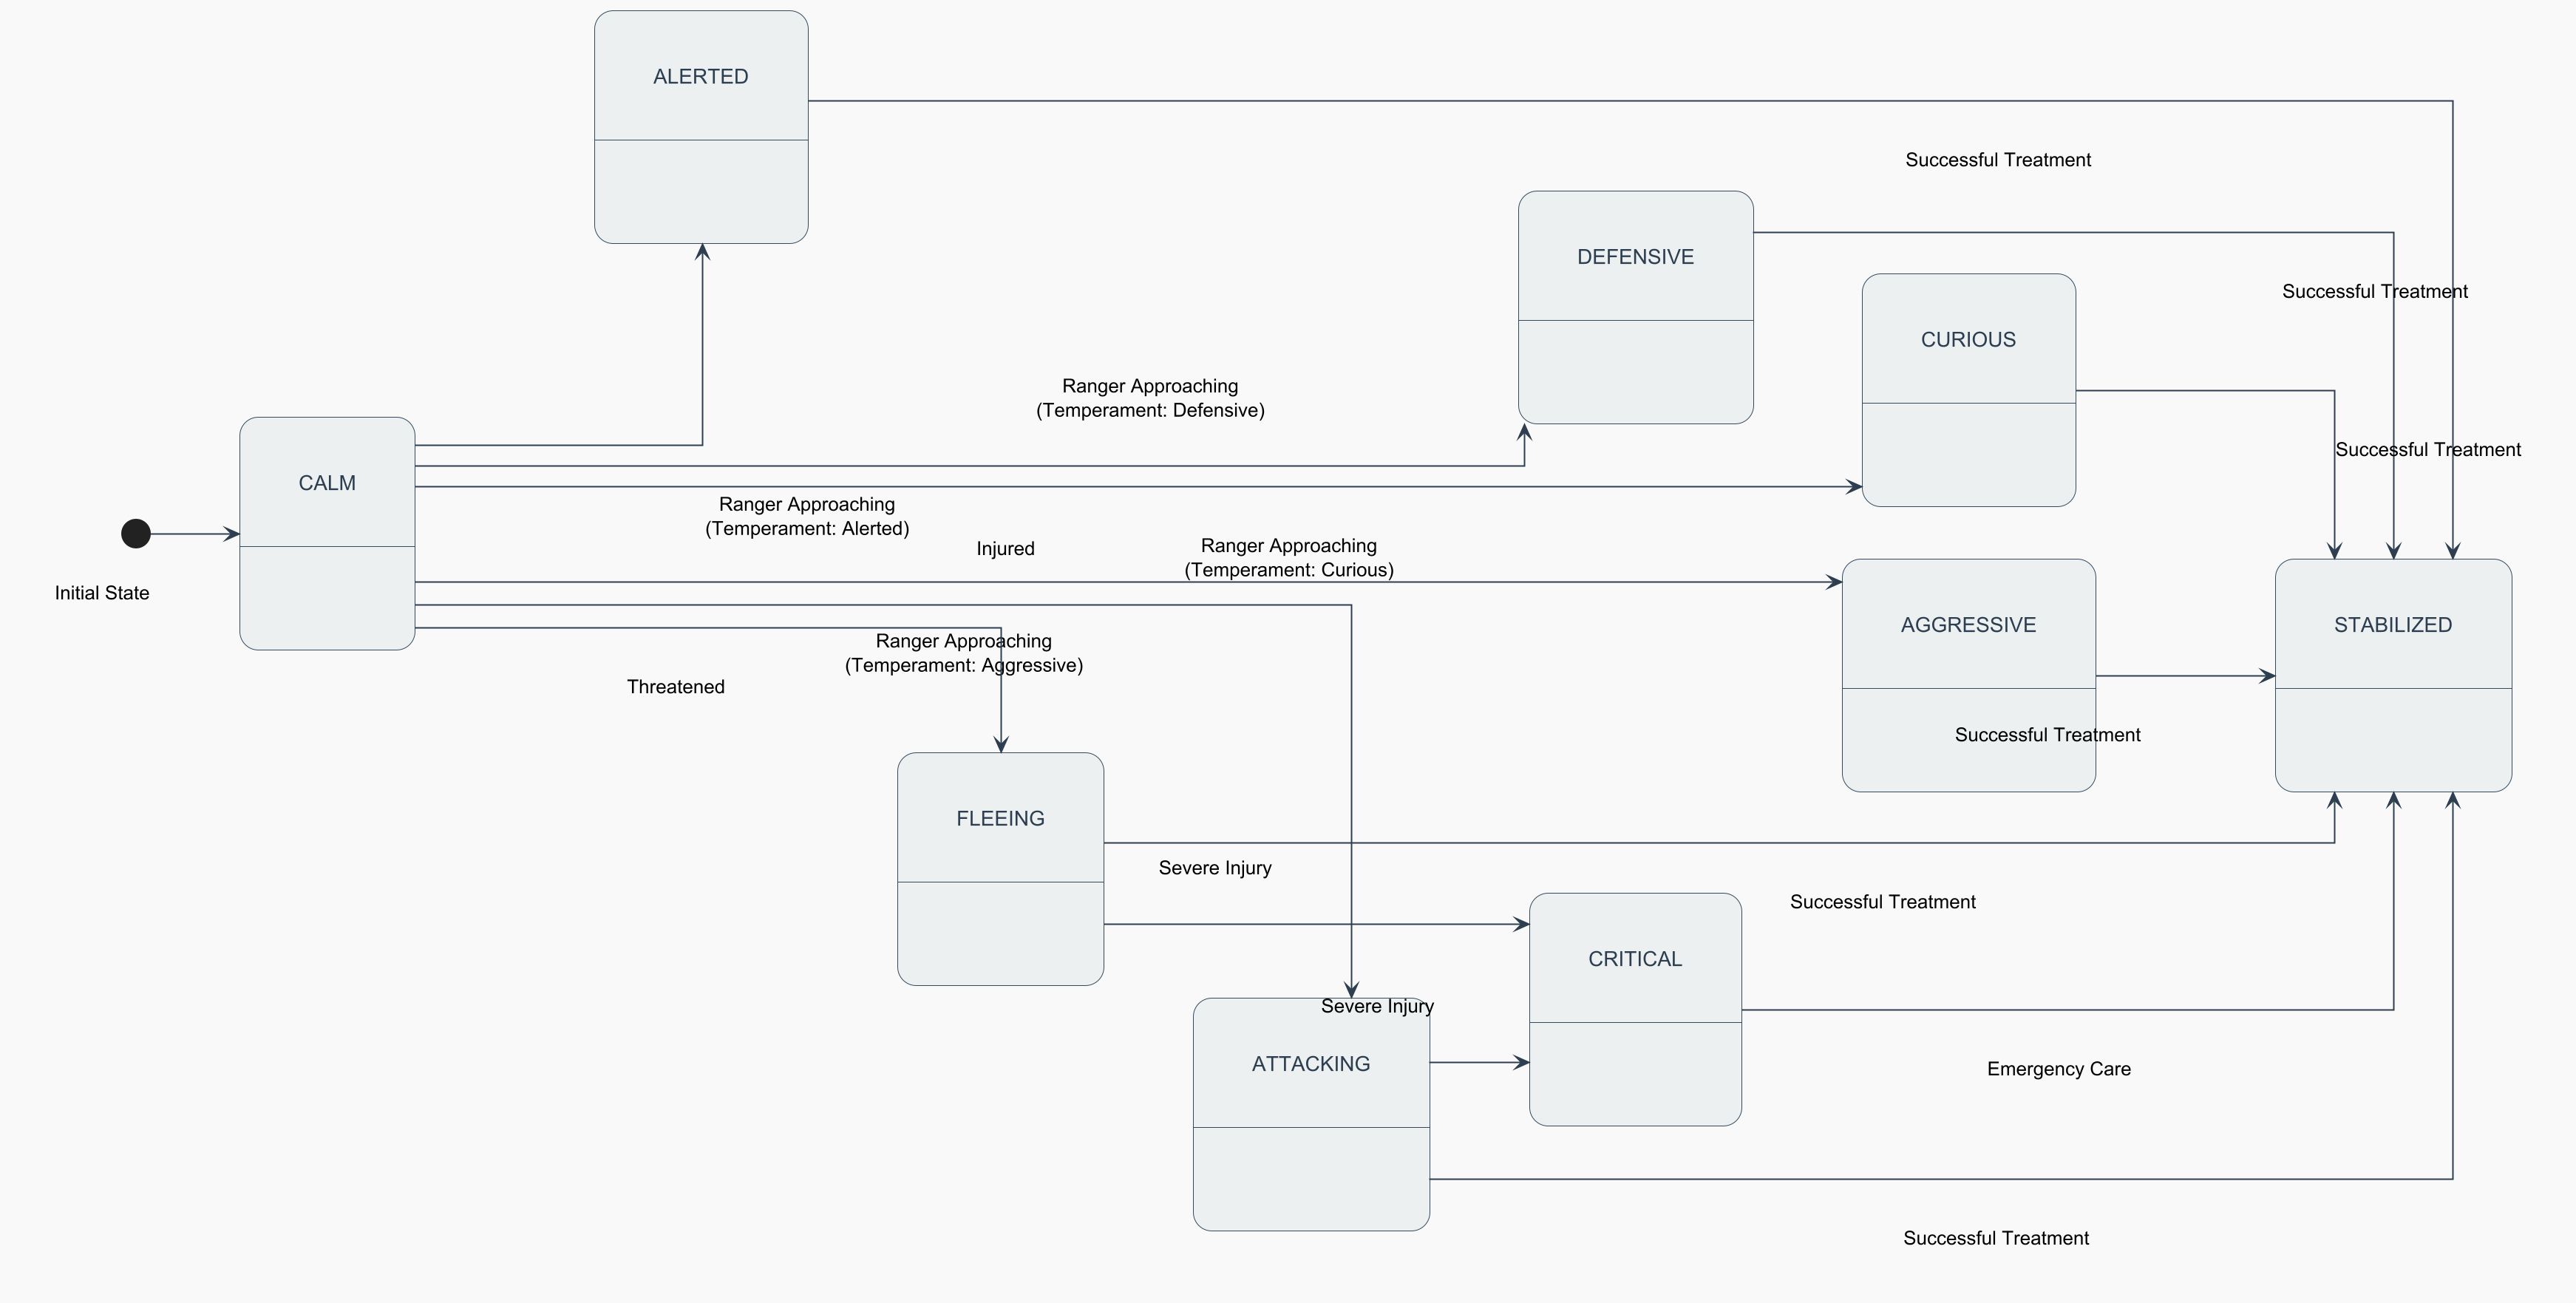
\includegraphics[width=0.8\textwidth]{state-diagram.png}
    \caption{Animal state diagram}
    \label{fig:animal-state-diagram}
\end{figure}

\end{document}